\documentclass{scrreprt}

\usepackage{aligned-overset}
\usepackage{amsmath}
\usepackage{amsthm}
\usepackage{amssymb}
\usepackage{bm}
\usepackage[inline,shortlabels]{enumitem}
\usepackage{hyperref}
\usepackage[utf8]{inputenc}
\usepackage{multicol}
\usepackage{mathtools}
\usepackage{pdflscape}
\usepackage{physics}
\usepackage{tabularx}
\usepackage[table]{xcolor}
\usepackage{titling}
\usepackage{fancyhdr}
\usepackage{xfrac}
\usepackage{pgfplots}

\pgfplotsset{compat = newest}
\usepgfplotslibrary{fillbetween}
\usetikzlibrary{calc}


\author{Karsten Lehmann}
\date{SoSe 2025}
\title{Übungsblatt 03\\INF-B-260, Informations- und Kodierungstheorie}

\newcommand{\ld}{\text{ld}}

\setlength{\parindent}{0pt}

\setlength{\headheight}{26pt}
\pagestyle{fancy}
\fancyhf{}
\lhead{\thetitle}
\rhead{\theauthor}
\lfoot{\thedate}
\rfoot{Seite \thepage}

\begin{document}
\paragraph{Ü 3.1 Diskrete Kanalmodelle}
\begin{enumerate}[1.]
\item Gegeben sei ein symmetrisch gestörter Binärkanal mit der
  Schrittfehlerwahrscheinlichkeit  $p_s = 0.1$.

  Bestimmen Sie die Traninformation dieses Kanals bei folgenden
  Wahrscheinlichkeitsverteilungen der angeschlossenen Quellen:

  \begin{enumerate}[(a)]
  \item $p\qty\big(x_0) = p\qty\big(x_1) = 0.5$

    \subparagraph{Lsg.} Es ist

    \begin{tikzpicture}
      \node (x0) at (0, 0) {$0.5 = p\qty\big(x_0)$};
      \node (x1) at (0, -2) {$0.5 = p\qty\big(x_1)$};
      \node (y0) at (6, 0) {$p\qty\big(y_0) = 0.5$};
      \node (y1) at (6, -2) {$p\qty\big(y_1) = 0.5$};

      \draw[->] (x0) -- node[above, midway] {0.9} (y0);
      \draw[->] (x0) -- node[above, midway, xshift=-1cm, yshift=0.4cm] {0.1} (y1);
      \draw[->] (x1) -- node[above, midway, xshift=-1cm, yshift=-0.9cm] {0.1} (y0);
      \draw[->] (x1) -- node[above, midway, yshift=-0.7cm] {0.9} (y1);
    \end{tikzpicture}

    und somit
    \begin{flalign*}
      H\qty\big(y) &= \ld 2 = 1 \frac{\text{bit}}{\text{KZ}} \\
      H\qty\big(y|x) &= \sum_{i = 1}^z \sum_{j = 1}^z p\qty\big(x_i)p\qty\big(y_j|x_i) \ld \frac{1}{p\qty\big(y_j|x_i)} \\
                   &= p\qty\big(x_0)p\qty\big(y_0 | x_0) \ld \frac{1}{p\qty\big(y_0 | x_0)}
                     + p\qty\big(x_0)p\qty\big(y_1 | x_0) \ld \frac{1}{p\qty\big(y_1 | x_0)} + \\
                   &\quad p\qty\big(x_1)p\qty\big(y_0 | x_1) \ld \frac{1}{p\qty\big(y_0 | x_1)}
                     + p\qty\big(x_1)p\qty\big(y_1 | x_1) \ld \frac{1}{p\qty\big(y_1 | x_1)} \\
                   &= 0.5 \cdot 0.9 \ld \frac{1}{0.9}
                     + 0.5 \cdot 0.1 \ld \frac{1}{0.1}
                     + 0.5 \cdot 0.1 \ld \frac{1}{0.1}
                     + 0.5 \cdot 0.9 \ld \frac{1}{0.9} \\
                   &\approx 0.469 \frac{\text{bit}}{\text{KZ}} \\
      H_q &= H\qty\big(y) - H\qty\big(y|x) = 1 \frac{\text{bit}}{\text{KZ}} - 0.469 \frac{\text{bit}}{\text{KZ}} \\
                   &= 0.531 \frac{\text{bit}}{\text{KZ}}
    \end{flalign*}
  \end{enumerate}

\newpage
\item Das Übertragungsverhalten eines Binärkanals sei durch folgende
  Wahrscheinlichkeiten bestimmt:
  $p\qty\big(y_0|x_0) = 0.5; \; p\qty\big(x_1|y_1) = 1;\;$
  $p\qty\big(y_1|x_0) = 0.5$.

  Es ist die Transformation für folgende Zustandswahrscheinlichkeiten am
  Kanaleingang zu berechnen:
  \begin{enumerate}[(a)]
  \setcounter{enumii}{1}
  \item $p\qty\big(1) = \frac{1}{5}$

    \subparagraph{Lsg.} Es ist

    \begin{tikzpicture}
      \node (x0) at (0, 0) {$\frac{1}{5} = p\qty\big(x_0)$};
      \node (x1) at (0, -2) {$\frac{4}{5} = p\qty\big(x_1)$};
      \node (y0) at (6, 0) {$p\qty\big(y_0) = 0.6$};
      \node (y1) at (6, -2) {$p\qty\big(y_1) = 0.4$};

      \draw[->] (x0) -- node[above, midway] {1} (y0);
      \draw[->] (x0) -- node[above, midway, xshift=-1cm, yshift=0.3cm] {0} (y1);
      \draw[->] (x1) -- node[above, midway, xshift=-1cm, yshift=-1.5cm] {0.5} (y0);
      \draw[->] (x1) -- node[above, midway, xshift=-1cm, yshift=0.1cm] {0.5} (y1);
    \end{tikzpicture}

    und somit

    \begin{flalign*}
      H\qty\big(y) &= \sum_{i = 1}^2 p\qty\big(y_i) \ld \frac{1}{p\qty\big(y_i)}
                    = 0.4 \cdot \ld \frac{1}{0.4} + 0.6 \cdot \ld \frac{1}{0.6} \\
                   &\approx 0.971 \frac{\text{bit}}{\text{KZ}} \\
      H\qty\big(y|x) &= \sum_{i = 1}^z \sum_{j = 1}^z p\qty\big(x_i)p\qty\big(y_j|x_i) \ld \frac{1}{p\qty\big(y_j|x_i)} \\
                   &= p\qty\big(x_0)p\qty\big(y_0 | x_0) \ld \frac{1}{p\qty\big(y_0 | x_0)}
                     + p\qty\big(x_0)p\qty\big(y_1 | x_0) \ld \frac{1}{p\qty\big(y_1 | x_0)} + \\
                   &\quad p\qty\big(x_1)p\qty\big(y_0 | x_1) \ld \frac{1}{p\qty\big(y_0 | x_1)}
                     + p\qty\big(x_1)p\qty\big(y_1 | x_1) \ld \frac{1}{p\qty\big(y_1 | x_1)} \\
                   &= 0.2 \cdot 1 \ld \frac{1}{1}
                     + 0.2 \cdot 0
                     + 0.8 \cdot 0.5 \ld \frac{1}{0.5}
                     + 0.8 \cdot 0.5 \ld \frac{1}{0.5} \\
                   &= 0.8 \frac{\text{bit}}{\text{KZ}} \\
      H_q &= H\qty\big(y) - H\qty\big(y|x) = 0.971 \frac{\text{bit}}{\text{KZ}} - 0.8 \frac{\text{bit}}{\text{KZ}} \\
                   &= 0.171 \frac{\text{bit}}{\text{KZ}}
    \end{flalign*}
  \end{enumerate}

\newpage
\setcounter{enumi}{4}
\item Ein Sender soll über ein Alphabet von 5 Symbolen $x_1, x_2, \ldots, x_5$
  verfügen,
  während das Alphabet des entsprechenden Empfängers nur 4 Symbole $y_1, y_2, y_3$
  und $y_4$ enthält.

  Bekannt ist die Matrix der Verbundwahrscheinlichkeiten
  \[
    \qty(p\qty\big(x_1, y_i)) = \begin{pmatrix}
      0.25 & 0    & 0.05 & 0    \\
      0    & 0    & 0.10 & 0    \\
      0    & 0    & 0.10 & 0    \\
      0.15 & 0.20 & 0    & 0    \\
      0    & 0    & 0    & 0.15 \\
    \end{pmatrix}
  \]
  Berechnen Sie die Transinformation!

  \subparagraph{Lsg.} Es sind die Auftrittswahrscheinlichkeiten der Quelle die
  Summen der Zeilen und die Auftrittswahrscheinlichkeiten des Empfängers die
  Summen der Spalten, also
  \begin{flalign*}
    p\qty\big(x_1) &= 0.3 \\
    p\qty\big(x_2) &= 0.1 \\
    p\qty\big(x_3) &= 0.1 \\
    p\qty\big(x_4) &= 0.35 \\
    p\qty\big(x_5) &= 0.15
  \end{flalign*}
  und
  \begin{flalign*}
    p\qty\big(y_1) &= 0.4 \\
    p\qty\big(y_2) &= 0.2 \\
    p\qty\big(y_3) &= 0.25 \\
    p\qty\big(y_4) &= 0.15
  \end{flalign*}

  \[
    \frac{\qty(p\qty\big(x_i, y_j))}{p\qty\big(x_i)} = \qty(p\qty\big(y_j | x_i))
    = \begin{pmatrix}
      \frac{0.25}{0.3}  & 0                & \frac{0.05}{0.3} & 0                 \\
      0                 & 0                & \frac{0.1}{0.1}  & 0                 \\
      0                 & 0                & \frac{0.1}{0.1}  & 0                 \\
      \frac{0.15}{0.25} & \frac{0.2}{0.25} & 0                & 0                 \\
      0                 & 0                & 0                & \frac{0.15}{0.15} \\
    \end{pmatrix}833
    = \begin{pmatrix}
      0.833 & 0     & 0.167 & 0 \\
      0     & 0     & 1     & 0 \\
      0     & 0     & 1     & 0 \\
      0.429 & 0.571 & 0     & 0 \\
      0     & 0     & 0    & 1 \\
    \end{pmatrix}
  \]

  und das Kanalmodell
  \begin{tikzpicture}
    \node (x1) at (0, 0) {$0.3 = p\qty\big(x_1)$};
    \node (x2) at (0, -2) {$0.1 = p\qty\big(x_2)$};
    \node (x3) at (0, -4) {$0.1 = p\qty\big(x_3)$};
    \node (x4) at (0, -6) {$0.35 = p\qty\big(x_4)$};
    \node (x5) at (0, -8) {$0.15 = p\qty\big(x_5)$};
    \node (y1) at (6, -1) {$p\qty\big(y_1) = 0.4$};
    \node (y2) at (6, -3) {$p\qty\big(y_2) = 0.2$};
    \node (y3) at (6, -5) {$p\qty\big(y_3) = 0.25$};
    \node (y4) at (6, -7) {$p\qty\big(y_4) = 0.15$};

    \draw[->] (x1) -- node[above, pos=0.25] {0.833} (y1);
    \draw[->] (x1) -- node[above, pos=0.25] {0.167} (y3);
    \draw[->] (x2) -- node[above, pos=0.25] {1} (y3);
    \draw[->] (x3) -- node[above, pos=0.25] {1} (y3);
    \draw[->] (x4) -- node[below, pos=0.25] {0.429} (y1);
    \draw[->] (x4) -- node[below, pos=0.25] {0.571} (y2);
    \draw[->] (x5) -- node[above, pos=0.25] {1} (y4);
  \end{tikzpicture}
\end{enumerate}

\newpage
\paragraph{Zusatzaufgabe} Es ist folgendes Kanalmodell gegeben
(AZ steht für Auslöschungszeichen):

\begin{tikzpicture}
  \node (x1) at (0, -1) {$0.5 = p\qty\big(x_1)$};
  \node (x0) at (0, -3) {$0.5 = p\qty\big(x_0)$};
  \node (y1) at (6, 0) {$p\qty\big(y_1)$};
  \node at (8.2, 0) {$= \frac{1}{2} \epsilon + \frac{1}{2} \qty\big(1 - \epsilon - \delta)$};
  \node at (7.45, -0.8) {$= \frac{1}{2} \qty\big(1 - \delta)$};
  \node (az) at (6, -2) {$p\qty\big(\text{AZ})$};
  \node at (7.85, -2) {$= \frac{1}{2} \delta + \frac{1}{2} \delta = \delta$};
  \node (y0) at (6, -4) {$p\qty\big(y_0)$};
  \node at (8.2, -4) {$= \frac{1}{2} \epsilon + \frac{1}{2} \qty\big(1 - \epsilon - \delta)$};
  \node at (7.2, -4.8) {$= p\qty\big(y_1)$};

  \draw[->] (x1) -- node[above, pos=0.25] {$1 - \epsilon - \delta$} (y1);
  \draw[->] (x1) -- node[above, pos=0.25] {$\delta$} (az);
  \draw[->] (x1) -- node[above, pos=0.1] {$\epsilon$} (y0);
  \draw[->] (x0) -- node[above, pos=0.25] {$1 - \epsilon - \delta$} (y0);
  \draw[->] (x0) -- node[above, pos=0.25] {$\delta$} (az);
  \draw[->] (x0) -- node[above, pos=0.1] {$\epsilon$} (y1);
\end{tikzpicture}

Die Rechnung dazu:
\begin{flalign*}
  H\qty\big(y) &= \underset{y_0, \; y_1}{\underbrace{2 \cdot \frac{1}{2} \qty\big(1 - \delta) \ld \frac{1}{\frac{1}{2} \qty\big(1 - \delta)}}} + \underset{\text{AZ}}{\underbrace{\delta\ld\frac{1}{\delta}}} \\
               &= \qty\big(1 - \delta)\ld\qty\big(2) + \qty\big(1 - \delta)\ld\frac{1}{1 - \delta} + \delta\ld\frac{1}{\delta} \\
  H\qty\big(y|x) &= 2\frac{1}{2} \qty(\qty(1 - \epsilon - \delta)\ld\frac{1}{1 - \epsilon - \delta} + \delta\ld\frac{1}{\delta} + \epsilon\ld\frac{1}{\epsilon}) \\
               &= \qty(1 - \epsilon - \delta)\ld\frac{1}{1 - \epsilon - \delta} + \delta\ld\frac{1}{\delta} + \epsilon\ld\frac{1}{\epsilon} \\
  H_T &= \qty\big(1 - \delta) + \qty\big(1 - \delta)\ld\frac{1}{1 - \delta} + \delta\ld\frac{1}{\delta} - \qty\big(1 - \epsilon - \delta)\ld\frac{1}{1 - \epsilon - \delta} - \delta\ld\frac{1}{\delta} - \epsilon\ld\frac{1}{\epsilon} \\
               &= \qty\big(1 - \delta) + \qty\big(1 - \delta)\ld\frac{1}{1 - \delta} - \qty\big(1 - \epsilon - \delta)\ld\frac{1}{1 - \epsilon - \delta} - \epsilon\ld\frac{1}{\epsilon}
\end{flalign*}


\end{document}
